\documentclass[12pt,a4paper,bibliography=totocnumbered,listof=totocnumbered]{scrartcl}

\usepackage[english]{babel}
\usepackage[utf8]{inputenc}
\usepackage{amsmath}
\usepackage{amsfonts}
\usepackage{amssymb}
\usepackage{graphicx}
\usepackage{fancyhdr}
\usepackage{tabularx}
\usepackage{geometry}
\usepackage{setspace}
\usepackage[right]{eurosym}
\usepackage[printonlyused]{acronym}
\usepackage{subfig}
\usepackage{floatflt}
\usepackage[usenames,dvipsnames]{color}
\usepackage{colortbl}
\usepackage{color}
\usepackage{paralist}
\usepackage{array}
\usepackage{titlesec}
\usepackage{parskip}
\usepackage[right]{eurosym}
\usepackage[subfigure,titles]{tocloft}
\usepackage[pdfpagelabels=true]{hyperref}
\usepackage{units}
\usepackage{booktabs}
\usepackage{listings}
\usepackage{float}
\usepackage{bold-extra}
\lstset{mathescape=true,
        %frame=tB,
        numbers=left, 
        numberstyle=\tiny,
        basicstyle=\ttfamily\footnotesize, 
        numbers=left,
        morekeywords={Input, for, in},
        keywordstyle = \bfseries,
        xleftmargin=.04\textwidth, 
        captionpos=b,
        breaklines=true, 
        showstringspaces=false, 
        tabsize=2, 
        frame=shadowbox}
\renewcommand{\lstlistingname}{Algorithmus}% Listing -> Algorithm
\captionsetup[lstlisting]{font={small}}
\makeatletter
\def\l@lstlisting#1#2{\@dottedtocline{1}{0em}{1em}{\hspace{1,5em} Lst. #1}{#2}}
\makeatother

\geometry{a4paper, top=25mm, left=20mm, right=20mm, bottom=25mm, headsep=10mm, footskip=12mm}


\graphicspath{{../Figures/}}

\hypersetup{unicode=false, pdftoolbar=true, pdfmenubar=true, pdffitwindow=false, pdfstartview={FitH},
	pdftitle={Ausarbeitung Evolutionsstrategien als Alternative zu Bestärkendem Lernen im Bereich der Künstlichen Intelligenz},
	pdfauthor={Daniela Schacherer},
	pdfsubject={Seminararbeit},
	pdfcreator={\LaTeX\ with package \flqq hyperref\frqq},
	pdfproducer={pdfTeX \the\pdftexversion.\pdftexrevision},
	pdfkeywords={Seminararbeit},
	pdfnewwindow=true,
	colorlinks=true,linkcolor=black,citecolor=black,filecolor=magenta,urlcolor=black}
\pdfinfo{/CreationDate (D:20110620133321)}
\newcommand*{\source}{%
  \footnotesize Source:
  }

\begin{document}

\titlespacing{\section}{0pt}{12pt plus 4pt minus 2pt}{-6pt plus 2pt minus 2pt}

% Kopf- und Fusszeile
\renewcommand{\sectionmark}[1]{\markright{#1}}
\renewcommand{\leftmark}{\rightmark}
\pagestyle{fancy}
\lhead{}
\chead{}
\rhead{\thesection\space\contentsname}
\cfoot{}
\rfoot{\thepage}
\renewcommand{\headrulewidth}{0.4pt}
\renewcommand{\footrulewidth}{0.4pt}

% Vorspann
\renewcommand{\thesection}{\Roman{section}}
\renewcommand{\theHsection}{\Roman{section}}
\pagenumbering{Roman}

% %----------------------------------------------------------------------------------------
%	TITLE PAGE
%----------------------------------------------------------------------------------------

\begin{titlepage}

\newcommand{\HRule}{\rule{\linewidth}{0.5mm}} % Defines a new command for the horizontal lines, change thickness here

\center % Center everything on the page

\LARGE Ruprecht-Karls-University Heidelberg \\[0.5cm] % Name of your university/college
\Large Faculty of Mathematics and Computer Science \\[1.5cm]
\Large \textbf{Project}: Object Recognition and Image Understanding\\[0.5cm] % Major heading such as course name

\HRule \\[0.4cm]
{ \textsc{\huge \bfseries Traffic Sign Detection in Colour Images}}\\ \textsc{\Large two approaches in comparison}\\[0.4cm] % Title of your document
\HRule \\[1.5cm]

\begin{minipage}{0.4\textwidth}
\begin{flushleft} \large
\emph{Author:}\\
Daniela Schacherer, 3165890, M.Sc. Angewandte Informatik \\
Marvin Klaus, 3486809, M.Sc. Angewandte Informatik \\% Your name
\end{flushleft}

\begin{flushleft} \large
\emph{Lecturer:}\\
Prof. Björn Ommer \\ % Your name
\end{flushleft}

\begin{flushleft} \large
\emph{Date}\\
24.07.2018 \\% Your name
\end{flushleft}

\end{minipage}
~
\begin{minipage}{0.4\textwidth}
\end{minipage}\\[4cm]

\vfill % Fill the rest of the page with whitespace

\end{titlepage}

%----------------------------------------------------------------------------------------
%	INHALTSVERZEICHNIS
%----------------------------------------------------------------

\tableofcontents % Include a table of contents

\newpage % Begins the essay on a new page instead of on the same page as the table of contents 


% ----------------------------------------------------------------------------------------------------------
% Inhalt
% ----------------------------------------------------------------------------------------------------------
% Abstände Überschrift
\titlespacing{\section}{0pt}{12pt plus 4pt minus 2pt}{-6pt plus 2pt minus 2pt}
\titlespacing{\subsection}{0pt}{12pt plus 4pt minus 2pt}{-6pt plus 2pt minus 2pt}
\titlespacing{\subsubsection}{0pt}{12pt plus 4pt minus 2pt}{-6pt plus 2pt minus 2pt}

% Kopfzeile
\renewcommand{\sectionmark}[1]{\markright{#1}}
\renewcommand{\subsectionmark}[1]{}
\renewcommand{\subsubsectionmark}[1]{}
\lhead{Chapter \thesection}
\rhead{\rightmark}

\onehalfspacing
\renewcommand{\thesection}{\arabic{section}}
\renewcommand{\theHsection}{\arabic{section}}
\setcounter{section}{0}
\pagenumbering{arabic}
\setcounter{page}{1}


\section{Introduction}
Autonomous driving is nowadays one of the most growing research fields. In this context visual detection and recognition of road signs becomes particularly important. The project presented in this report aims at the exploration of two state-of-the-art approaches towards the detection of traffic signs in color images. In contrast to traffic sign recognition, detection aims merely at locating the traffic signs in the images, however, not at classifying them. 

\section{Dataset}
The dataset employed for this task was made publicly available by the University of Bochum as part of a traffic sign detection competition in 2013 \cite{dataset}. The data set comprises 900 images (1360 $\times$ 800 pixels) in PPM format containing 1206 traffic signs. Additionally, the image sections containing only the traffic signs and a CSV file containing ground truth information (location of the traffic signs within the images) are provided. Each image contains zero to six of those traffic signs included in the competition like, for example, speed limit or stop signs. For a complete list of the competition relevant categories see Appendix A. The sizes of the traffic signs in the images vary from $16$ to $128$ pixels w.r.t the longer edge \cite{Houben-IJCNN-2013}. \\
The images were collected such that different street scenes as urban, rural, or highway as well as different lightning and weather conditions  are equally represented in the dataset. Figure \ref{fig:ex_images} shows some examples contained in the data set. \cite{Houben-IJCNN-2013}.
\begin{figure}[H]
  \centering
  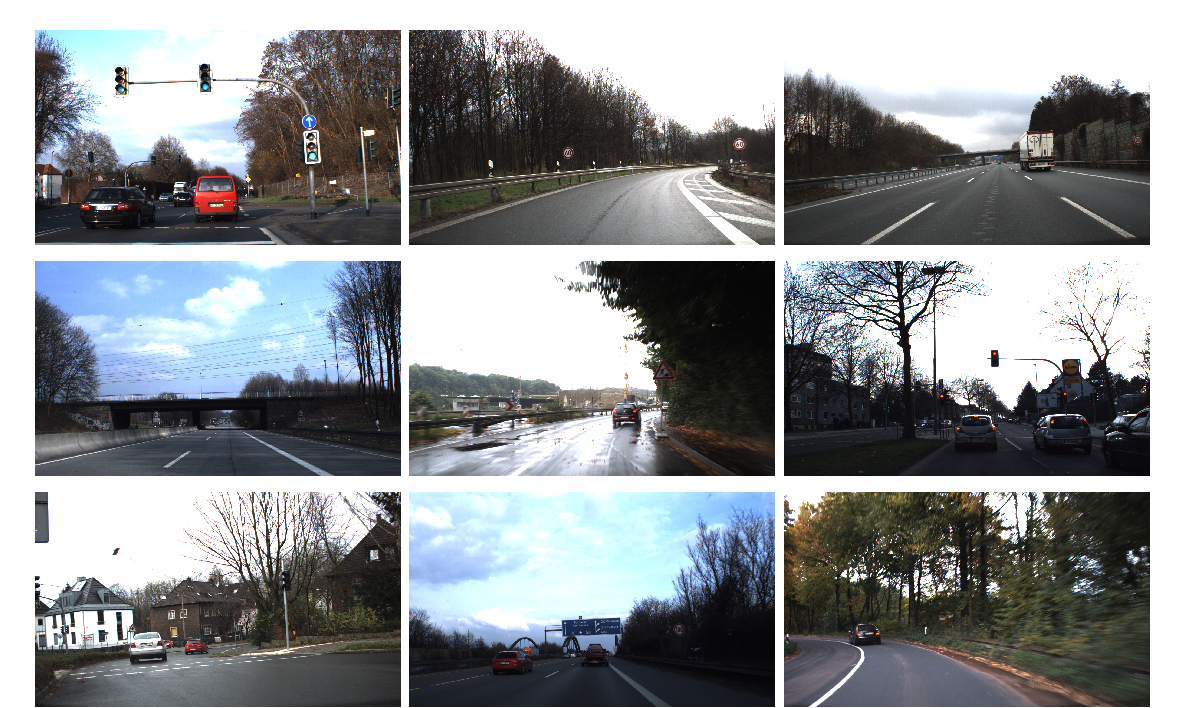
\includegraphics[width=\textwidth]{ex_imgs_smaller.png}
  \caption{Example images from the dataset.}
  \label{fig:ex_images}
\end{figure}

\section{First approach: Support Vector Machine \small{(Daniela)}} 
In the first approach we use a linear support vector machine (SVM) based on Histogram of oriented gradient (HOG) features to detect traffic signs in colour images. This combination is often used for object detection since HOG descriptors were introduced by Dalal and Triggs in 2005 \cite{Dalaltriggs}.
First, the SVM is trained to distinguish image patches showing traffic signs from image patches showing something else. For detection of road signs in a given image, a window is slided across the image at different scales employing the SVM for every image section. 

\subsection{Data preprocessing}
The training set was randomly divided into 600 images for training and 300 images for testing. 

\textbf{Positive training samples} \\
All traffic signs were extracted from the training set images using the ground truth locations provided. As the ground truth bounding boxes are not necessarily quadratic, they were converted to a quadratic shape by taking the larger side length and enlarging the smaller one equally in both directions. The extracted patches were then resized to a size of $30 \times 30$ pixels.  

\textbf{Negative training samples} \\
The easiest way to generate a "starter" set of negative samples was to take some images from the training set which do not show any sign. $30 \times 30 $ pixel sized patches were extracted from these images using a stepping window. A stepping window was preferred over a sliding one in order to avoid the negative samples being statistically dependent on each other. For a start, we sampled $5000$ negative image patches.

Some positive patches showing a traffic sign, as well as some of the negative patches, showing something else, are depicted in Figure \ref{fig:posnegpatch}. 

\begin{figure}[H]
\centering
  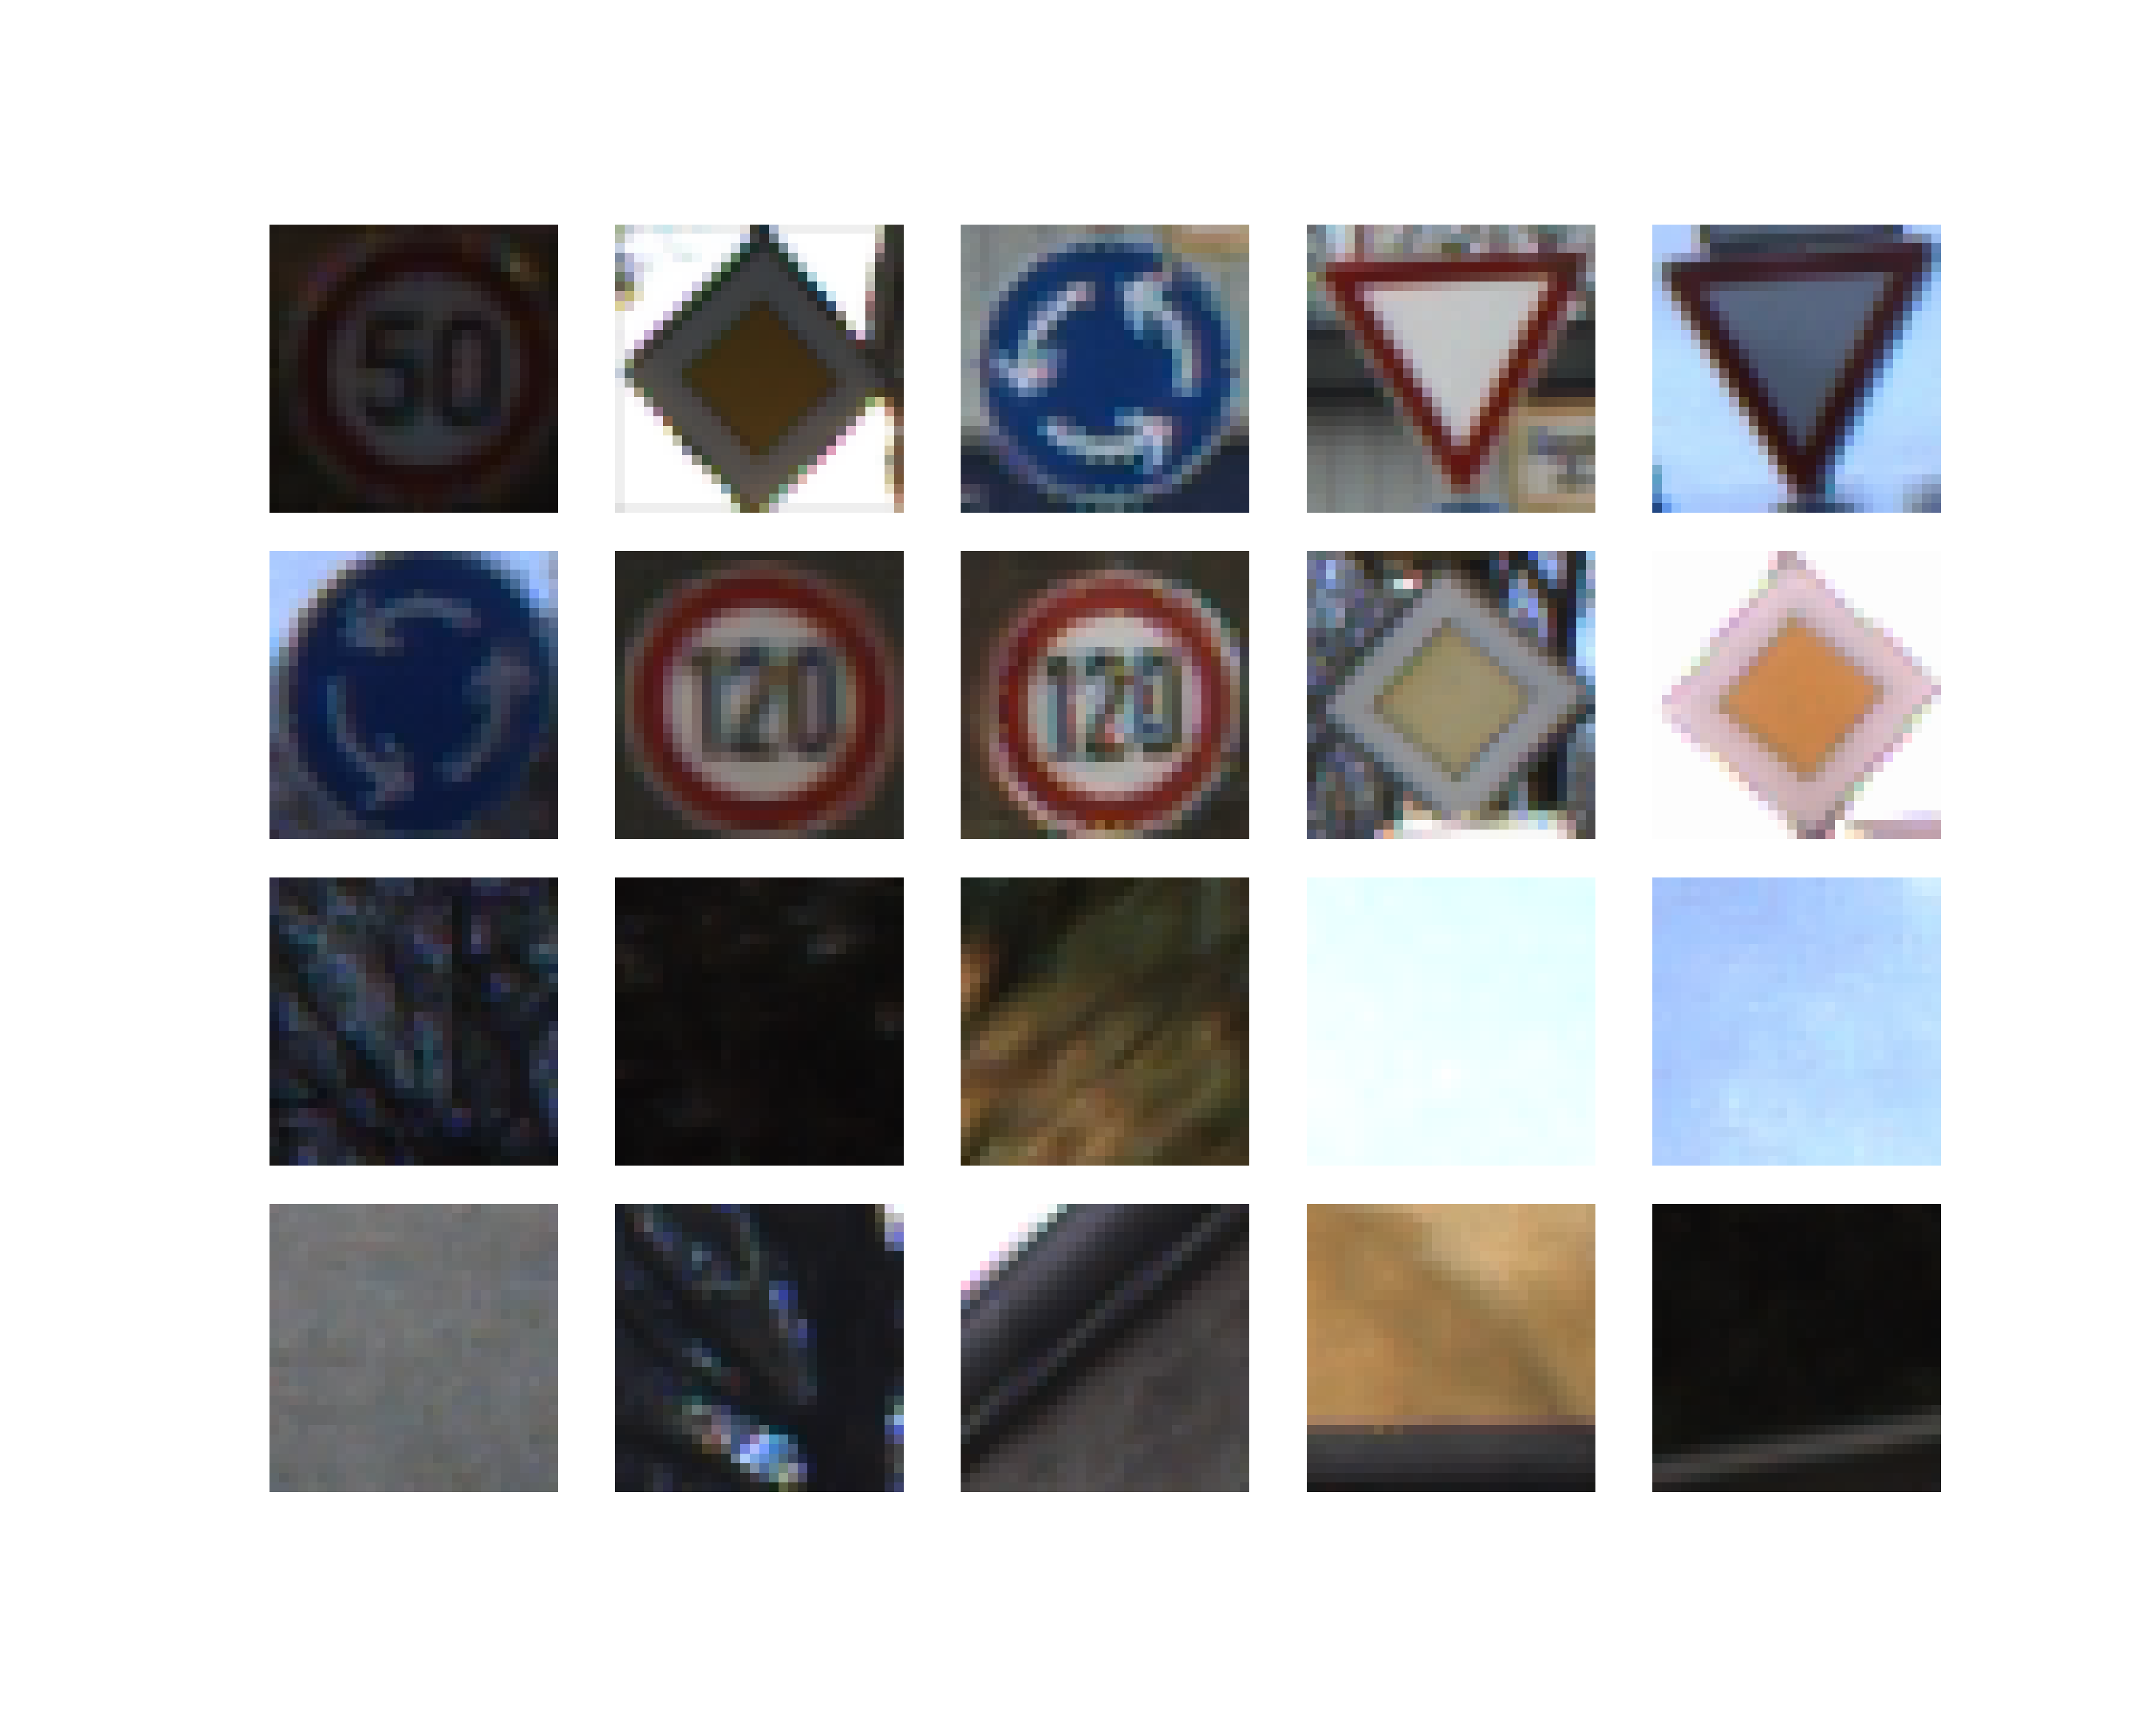
\includegraphics[width=0.6\linewidth]{pos_neg_patches.png}
  \caption{The first and second row show positive patches containing traffic signs, the third and fourth row show negative patches without a traffic sign contained. The size of all patches is $30 \times 30$ pixels.}
  \label{fig:posnegpatch}
\end{figure}


\subsection{Feature extraction using HOG}

\subsubsection{Theory HOG}
The \textbf{H}istogram of \textbf{O}riented \textbf{G}radients (HOG) is a feature descriptor widely used in the context of object detection. This method basically summarizes gradient orientations in localized sections of an image by performing the following five steps \cite{Dalal}: 

\begin{enumerate}
	\item Global image normalization using gamma compression: thereby one can compensate for variations in illumination or local shadowing effects.
	\item Computation of first order image gradients.
	\item Computation of gradient histograms: in so-called cells of predefined size (e.g. $5 \times 5$ pixels) gradient orientations over all pixels in the cell are accumulated in a histogram. 
	\item Normalization across blocks: as gradient strength must be locally normalized cells are grouped together into so-called blocks, on which normalization is performed. Possible methods for block normalization are, for instance, the L1-norm or the L2-norm.
	\item Collection of HOG descriptors from all cells into a combined feature vector. 
\end{enumerate}

\subsubsection{Application}
We used the HOG implementation from scikit-image \cite{scikithog}. As proposed by Houben \textit{et al.} who performed a similar approach, we considered 8 gradient orientations, used cells of size $5 \times 5$ pixels and a block size of $2 \times 2$ cells \cite{Houben-IJCNN-2013}. As block normalization method we chose the L2 normalization.
The final training set used to train the SVM is then constructed from the HOG features of the positive and negative patches. 

\subsection{Classification using SVM}
\subsubsection{Theory SVM}
A support vector machine is a well established supervised classification and regression method. Given a set of labeled training examples from two classes - positive and negative - a SVM training algorithm creates a model that can assign new examples to one category or the other. Formally, a SVM constructs a hyperplane by maximizing the margin between positive and negative data points (see Figure \ref{fig:svm}).  

\begin{figure}[H]
\centering
  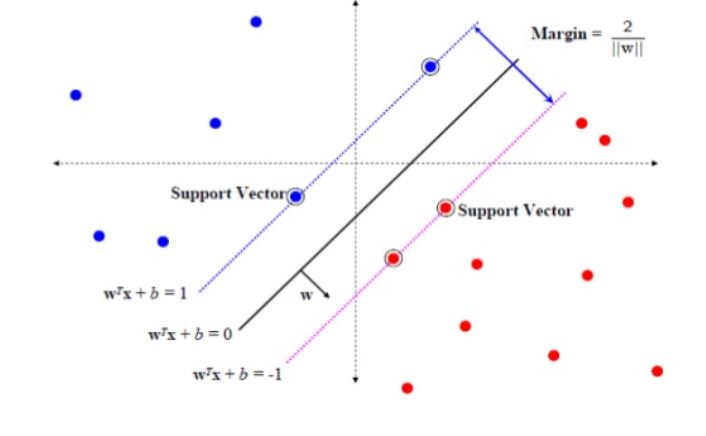
\includegraphics[width=0.7\linewidth]{svm.jpg}
  \caption{A Support Vector Machine tries to maximize the margin between positive and negative data points. Source: \url{https://www.slideshare.net/kambliruta/event-classification-prediction-using-support-vector-machine}}
  \label{fig:svm}
\end{figure}

\subsubsection{Training}
We used the SVM implementation provided by sklearn \cite{sklearnsvm} with the default values except for the kernel which we chose to be linear. With the intention to improve performance of the SVM as well as to obtain a sufficiently large training set, we additionally included a step of Hard Negative Mining (HNM). 
Therefore, the SVM is first trained with the previously constructed training set. Then, for every image and possible scale of the images dedicated for training, that contain no traffic sign, we apply the sliding window technique. At each window we compute the HOG descriptors and employ the pre-trained SVM. Each falsely detected patch is taken and explicitly added as a negative example to the training set. Finally, the SVM is retrained using the enlarged training set.
In the results section we compare the outcome with and without Hard Negative Mining based on the achieved training / test accuracies. \\
We expect a significant improvement when training with Hard Negative Mining as we obtain more variety in the negative training samples especially by using different scales of the images. Here we used $\sqrt(2)^i$ with $i = 0,...,-5$ as scale factor to obtain an image pyramid with $6$ layers including the original image. By the use of an image pyramid for Hard Negative Mining we can capture larger structures which might get confused easily with a traffic sign and explicitly learn the classifier to recognize them as negative examples.   

\subsubsection{Detection}
For detection of traffic signs in a given image we slide a window of size $30 \times 30$ pixels across the image at different scales - here we also used an image pyramid with  scale factor $\sqrt(2)^i$ where $i = 0,...,-5$ - and obtain a prediction for every image section from the SVM. If the thereby received regions possibly showing a traffic sign are obtained from another than the original scale of the image these are back computed to the original image's size. As a result we finally obtain a list of predicted bounding boxes relating to the original input image.

\subsubsection{Performance Measure} \label{ssec:perf}
For a quantitative measure of the detection performance each predicted bounding box $P$ is compared against every ground truth bounding box $G$ by means of the Jaccard similarity, which is defined as the intersection over union of the two bounding boxes: 
\begin{align*}
	S(P,G) = \frac{|P \cap G|}{|P \cup G|}
\end{align*}
If $S(P,G) \geq 0.5$ for any predicted bounding box $P$, the ground truth sign $G$ is considered as detected. In the end, we record the fraction of detected ground truth signs in all images (recall). \\
In addition, a measure for the amount signs detected erroneously - i.e. the false positive rate - is needed.  Therefore, we assess the fraction of predicted bounding boxes that have zero overlap with any of the ground truth bounding boxes. By computing $1-$ the false positive rate we yield the detection precision. 

\pagebreak
\section{Second Approach: R-CNN \small{(Marvin)}}

In the second approach we created a R-CNN to detect traffic signs in images. For this we first find all interesting regions in an image with the selective search algorithm and then use a CNN network to classify if there is an image in this region or not.

\subsection{Data preprocessing}

Before training the CNN we need to do some data preprocessing for this approach. The CNN will train and test with the help of the traffic sign images, classified to different types of signs by the creators of the dataset. Since we just want to distinguish between "no sign" and "sign", we collect them all together and use them as one single class of objects.\\Since the used dataset just offer traffic signs and no \textit{negative} training samples we need to create them. Similar like in the first approach, we filtered out all the traffic scene images without any traffic sign present. After that we took 32x32 parts from different images in random locations of the image. We collected 1000 negative samples through this approach.\\

\textbf{Improvement proposal:}\\
With more time left or a bigger group size there are several possible steps to improve the data preprocessing. For example as you can see in figure \ref{fig:data_hist} some traffic signs are less represented than others. To do something about this you could apply transformations on the images to rotate or tilt this traffic sign.\\
Also the collection of negative samples can be improved. For example you can collect these images more targeted like collect more shapes which look like signs but aren't or collect just a fraction of a sign. Also you can collect bigger pictures than 32x32 images and scale it down after that.

\subsection{Dataset creation}

With the preprocessed data we then create a dataset of these images. To make sure we have every traffic sign type in both the train and the test data, we split the images of every type in two parts where 0.3\% are test data and the rest train data. The results you can see in figure \ref{fig:data_hist} where the blue columns show the train data and the orange columns the test data. With this data we created two datasets for training and testing. For both all the images get resized to 32x32x3. One row in the finish dataset then looks like this: \{\textit{'image': image, 'id': sign-id, 'folder': image-folder}\}. The keys of the dictionary are self explanatory.

\begin{figure}[htbp] 
  \centering
     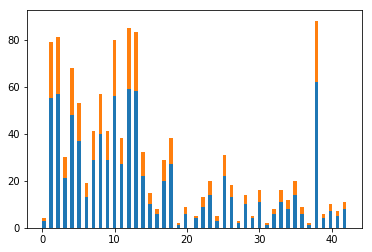
\includegraphics[width=0.7\textwidth]{data_hist}
  \caption{number of traffic signs by id divided by train and test data}
  \label{fig:data_hist}
\end{figure}

\subsection{CNN}

\textbf{Basics:}\\
A convolutional neural network (CNN) is artificial neural network which is used to analyzing and classifying images. A CNN consists essentially of filters (convolutional Layer) and aggregation layers (pooling Layer), which repeat alternately. At the end there are one or more fully connected layers to output the probability of different objects the image could represent.\\\\

\textbf{Architecture:}\\
To classify if there is a traffic sign in one image region we use a CNN. The network consists of two convolutional layers, both have a size of 5x5 where the first outputs 16 filters and the second layer 32. Both layers are follows by an normalization, ReLU and a pooling layer. After the convolutional layers we use fully connected layers to break the output down to two singles values.\\\\

\textbf{Training:}\\
To train the network we used the CrossEntropyLoss function. Since the output of the network consists of two values, the first should imply that there is no traffic sign in the image and the second one says that there is an image. With the Adam optimizer the accuracy of the network already looks really good after just 15 epochs. As you can see in \ref{fig:loss_acc} we got an accuracy of 94\%.

\begin{figure}[htbp] 
  \centering
     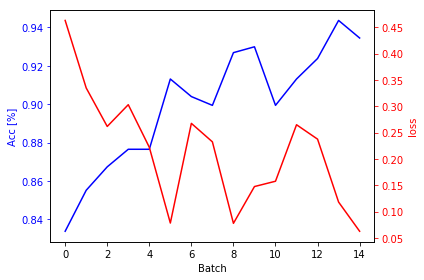
\includegraphics[width=0.7\textwidth]{loss_acc}
  \caption{loss and accuracy of net CNN}
  \label{fig:loss_acc}
\end{figure}

\subsection{Selective search}

Selective Search is a region proposal algorithm often used in object detection. It is based on computing hierarchical grouping of similar regions based on color, texture, size and shape compatibility.\\\\

Since we want to detect traffic signs in an image we first need to get some regions which we can classify with our CNN. For this reason we use the selective search algorithm which return bounding boxes of interesting regions in an image. While working with the selective search algorithm we noticed some issues with this algorithm. With the two parameters you can adjust, we found no perfect solution to find all the traffic signs in every image. At the end we took parameters where a good amount of traffic signs are represented in the interesting regions (scale=250, sigma=0.9). The network returns a huge amount of interesting regions for which reason we need to filter these regions. For example we just need regions which are in an certain size interval and are nearly quadratic. After this step an output of the selective search algorithm looks for example like in figure \ref{fig:selective_search_example}.

\begin{figure}[htbp] 
  \centering
     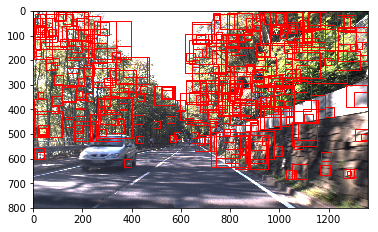
\includegraphics[width=0.7\textwidth]{selective_search_example}
  \caption{Example of the selective search algorithm after region filtering. All red rectangles are interesting regions.}
  \label{fig:selective_search_example}
\end{figure}

\subsection{Testing}

To get an accuracy of our traffic sign detector, we need to run all the found interesting regions in an image with our trained CNN. Like in the creation of datasets all of the regions need to be resized to a size of 32x32x3. After all regions of the wanted images are classified we need to examine how good our detection with the R-CNN works. For this we took the ground truth data and computed the Jaccard similarity for all the bounding boxes in the ground truth data and the regions which were classified as a traffic sign. A successful detection is then a similarity $\geq 0.5$. With this measurement the R-CNN gets an accuracy of just 32\%. This result is not really good, why is described in the discussion later on.

\pagebreak
\section{Results}
\subsection{First Approach \small{(Daniela)}}

The average detection performance measured by recall, precision and false positive rate on 30 randomly chosen images from the training respectively test set is reported in Table \ref{tab:perf}. Contrary to our expectations the prediction accuracy (recall) decreases when training the SVM with HNM. However, from precision and false positive values or when having a look at the bounding box predictions of the SVM trained with respectively without HNM, which are presented in Figure \ref{fig:compar}, one can see that Hard Negative Mining significantly lowers the false positive rate. On the left image both ground truth bounding boxes are detected, however there is a large amount of false positives. In the right image the second ground truth bounding box is not found, but the false positive rate is much lower. Due to the a better precision respectively lower false positive rate, we nevertheless assess Hard Negative Mining as an improvement and keep applying it when training our classifier.

\begin{table}[H]
\centering
\caption{Recall, precision and false positive rate on the train respectively test set obtained with and without HNM. For training and detection a sliding window of $30 \times 30$ pixels was used. The window's step size was $10$ pixels for training and $5$ pixels for detection.}
\small
  \begin{tabular}{l | c c c c c c}
  	  & 
      \multicolumn{3}{c}{\textbf{train acc}} &
      \multicolumn{3}{c}{\textbf{test acc}} \\
    & recall & precision & false positives & recall & precision & false positives \\ \toprule
    \textbf{w/o HNM} & 95.00\% & 15,09\% & 84,91\% & 99,17\% &6,29\% & 93,71\% \\
    \textbf{HNM}  & 84,73\% & 56,54\% & 43,46\% & 96,67\% & 51,11 & 48,99\% \\
  \end{tabular}
  \label{tab:perf}
\end{table}



\begin{figure}[H]
\begin{minipage}{0.48\textwidth}
\centering
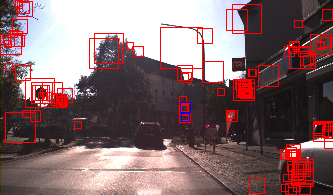
\includegraphics[width=\linewidth]{train102_wo_hn_prediction.png}
\end{minipage}
\hfill
\begin{minipage}{0.48\textwidth}
\centering
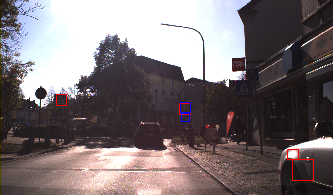
\includegraphics[width=\linewidth]{train102_predboxes2.png}
\end{minipage}
\caption{Bounding box prediction for the same image once using a SVM trained without HNM (left) and once trained with HNM (right). Ground truth bounding boxes are indicated in blue and predicted bounding boxes in red.}\label{fig:compar}
\end{figure}

In Figure \ref{fig:train_img_bbox} some training images are shown in which the ground truth bounding boxes are indicated in blue while the predicted bounding boxes are drawn in red. The respective detection performances are noted below. Almost all traffic signs - if present - are detected and there are only few false positive predictions. Especially interesting is the image in the upper middle: while the construction site sign is not detected possibly due to the poor lighting conditions, the hexagonal light spot in the upper left corner is recognized as a traffic sign instead. 

%% Result images test set
\begin{figure}[H]
\begin{minipage}{0.3\textwidth}
\centering
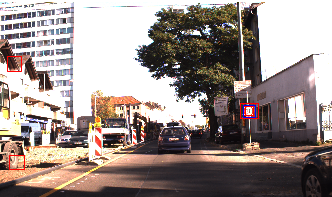
\includegraphics[width=\linewidth]{train0_predboxes2.png}
\small{(100\%)}
\end{minipage}
\hfill
\begin{minipage}{0.3\textwidth}
\centering
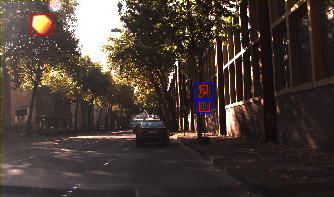
\includegraphics[width=\linewidth]{train23_predboxes2.png}
\small{(50\%)}
\end{minipage}
\hfill
\begin{minipage}{0.3\textwidth}
\centering
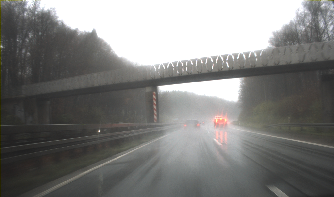
\includegraphics[width=\linewidth]{train212_predboxes2.png}
\small{(100\%)}
\end{minipage}

\begin{minipage}{0.3\textwidth}
\centering
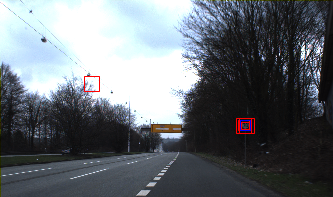
\includegraphics[width=\linewidth]{train407_predboxes2.png}
\small{(100\%)}
\end{minipage}
\hfill
\begin{minipage}{0.3\textwidth}
\centering
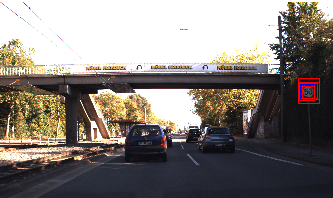
\includegraphics[width=\linewidth]{train599_predboxes2.png}
\small{(100\%)}
\end{minipage}
\hfill
\begin{minipage}{0.3\textwidth}
\centering
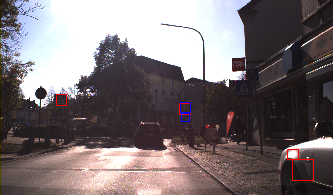
\includegraphics[width=\linewidth]{train102_predboxes2.png}
\small{(50\%)}
\end{minipage}
\caption{Images from the training set with ground truth bounding boxes in blue and predicted bounding boxes in red. Prediction accuracy in percentage according to the prediction measure explained in section \ref{ssec:perf} is given below each image.}
\label{fig:train_img_bbox}
\end{figure}

Figure \ref{fig:test_img_bbox} shows images from the test set along with ground truth and predicted bounding boxes. One can see that almost all traffic signs are detected as it was the case for the training images except for the rightmost sign in the upper middle image and the lower right image. If there is no traffic sign at all like in case of the bottom middle image, the algorithm does also recognize that correctly. However, the upper right and lower left image show that there are still sometimes false positives, which is not punished by our performance measure. Possibly the number of false positives can be reduced if another step of Hard Negative Mining is included.

%% Result images test set
\begin{figure}[H]
\begin{minipage}{0.3\textwidth}
\centering
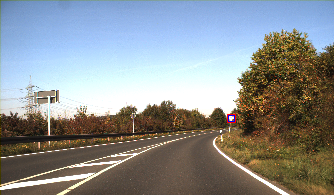
\includegraphics[width=\linewidth]{test2_wb_predboxes2.png}
\small{(100\%)}
\end{minipage}
\hfill
\begin{minipage}{0.3\textwidth}
\centering
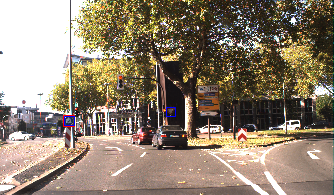
\includegraphics[width=\linewidth]{test14_wb_predboxes2.png}
\small{(50\%)}
\end{minipage}
\hfill
\begin{minipage}{0.3\textwidth}
\centering
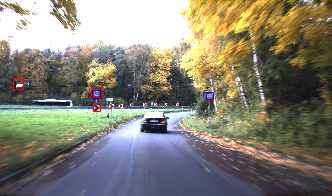
\includegraphics[width=\linewidth]{test44_wb_predboxes2.png}
\small{(100\%)}
\end{minipage}

\begin{minipage}{0.3\textwidth}
\centering
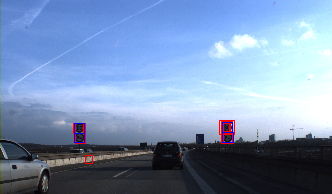
\includegraphics[width=\linewidth]{test144_wb_predboxes2.png}
\small{(100\%)}
\end{minipage}
\hfill
\begin{minipage}{0.3\textwidth}
\centering
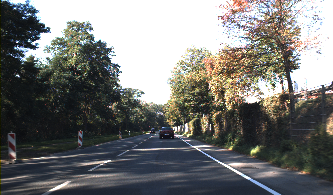
\includegraphics[width=\linewidth]{test200_wb_predboxes2.png}
\small{(100\%)}
\end{minipage}
\hfill
\begin{minipage}{0.3\textwidth}
\centering
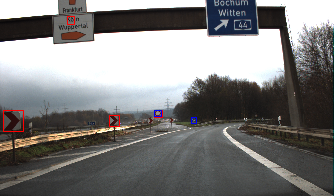
\includegraphics[width=\linewidth]{test100_wb_predboxes2.png}
\small{(50\%)}
\end{minipage}
\caption{Images from the test set with ground truth bounding boxes in blue and predicted bounding boxes in red. Prediction accuracy in percentage according to the prediction measure explained in section \ref{ssec:perf} is given below each image.}
\label{fig:test_img_bbox}
\end{figure}

Finally, we wanted to observe how the sliding window's step size during detection affects the performance. Figure \ref{fig:step_perf} plots the resulting performance against the detection step size. Already with very few data points it becomes clear that the detection step size is very critical to the success of traffic sign detection. 

\begin{figure}[H]
\centering
  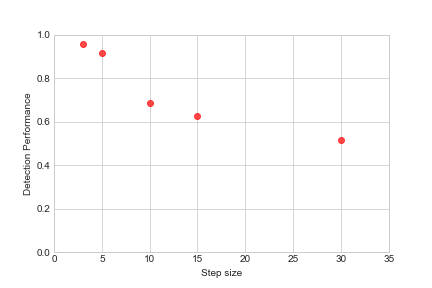
\includegraphics[width=0.5\linewidth]{step_performance_jaccthres0-5}
  \caption{Detection performance measured as recall on 30 randomly chosen images from the training set versus the step size of the sliding window used for detection.}
  \label{fig:step_perf}
\end{figure}

\pagebreak
\subsection{Second Approach \small{(Marvin)}}

\textbf{Network:}\\
The first thing we did was to train and test the CNN. The accuracy and loss function are displayed in figure <?>. We can see that the network can identify a traffic sign in approximately 94\% of cases. But we remember that we trained this network with the provided traffic signs of the dataset.\\\\

\textbf{Selective Search:}\\
Next we tried to get all interesting regions in a traffic scene image to classify each of these regions with our network. Figure <?> shows an example output of this algorithm. We can see, that in this image some traffic signs are recognized and some are not. We tried several parameters for the selective search algorithm but couldn't find a perfect setting to recognize all traffic signs in all images. Keep that in mind when looking at the results of the traffic sign detection.

\textbf{Detection:}\\
After getting all interesting regions in 40 random images, we classify each region with our CNN. We compared each region classified as traffic sign with the ground truth bounding box. The classification was successful if the two bounding boxes had a jaccard similarity $\geq 0.5$. The proportion of successful found traffic signs in the images are displayes in table <?>.\\
The results are a little bit surprising considering a CNN which recognized around 94\% of traffic sign images. Next we want to try to explain this phenomenon. 
\begin{enumerate}
\item As we saw in the results of the selective search algorithm, some traffic signs weren't even recognized and therefore not recognized which have a negative impact on the results. 
\item Also we looked at some images that were classified as traffic signs but were not counted as a successful detection. We saw some images which displayed a traffic sign but even with a good proprtion of the sign the jaccard similarity was less than $0.5$.
\item As we saw in figure <?> some traffic sign images are just underrepresented so that the network couldn't learn them good enough. This can affect the classification.
\end{enumerate}

With all these points we can explain the surprising bad results for the traffic sign detection with R-CNN's. But of course since simple R-CNN are a older approach there are better solutions to use for this problem. For example Fast R-CNN's and Faster R-CNN's are introduced which improve the region proposal computation. The Faster R-CNN for example introduce the Region Proposal Network which enables nearly cost-free region proposals.

\pagebreak
\section{Discussion}
To sum up the first approach, one can say that HOG features learned by a SVM are very well suited to detect traffic signs in color images. By the use of Hard Negative Mining the false positive rate can be lowered significantly, however, one looses some accuracy at the same time. An interesting idea could be to combine the predictions of a simply trained SVM with the ones from a HNM-trained SVM. Generally, the approach is very sensitive to the setting of the hyperparameters especially towards the step size of the sliding window for detection. The smaller the step size the better the detection performance - at the price to a much higher computational effort. It could thus be an improvement to use region of interest extraction instead of a sliding window, like for instance selective search. Another idea could be to include some image patches slightly overlapping with a traffic sign in the negative samples such that the classifier would get less easily confused by objects partly being similar to traffic signs. This could possibly further reduce the amount of false positive predictions. \\

\color{red} marvin \color{black}\\

In comparison, the SVM based on HOG features provides more convincing results than the R-CNN. Regarding computational effort the R-CNN is faster with the main bottleneck being the selective search algorithm. Faster R-CNNs provide one solution to this problem. They combine a region proposal network (RPN) with a R-CNN. The RPN is a fully convolutional network which is trained end-to-end to generate valuable region proposals, which are then used by the R-CNN for detection \cite{DBLP:journals/corr/RenHG015}. 




\pagebreak
\section{Appendix}
\subsection{Appendix A}
0 = speed limit 20 (prohibitory) \\
1 = speed limit 30 (prohibitory) \\
2 = speed limit 50 (prohibitory)\\
3 = speed limit 60 (prohibitory)\\
4 = speed limit 70 (prohibitory)\\
5 = speed limit 80 (prohibitory)\\
6 = restriction ends 80 (other)\\
7 = speed limit 100 (prohibitory)\\
8 = speed limit 120 (prohibitory)\\
9 = no overtaking (prohibitory)\\
10 = no overtaking (trucks) (prohibitory)\\
11 = priority at next intersection (danger)\\
12 = priority road (other)\\
13 = give way (other)\\
14 = stop (other)\\
15 = no traffic both ways (prohibitory)\\
16 = no trucks (prohibitory)\\
17 = no entry (other)\\
18 = danger (danger)\\
19 = bend left (danger)\\
20 = bend right (danger)\\
21 = bend (danger)\\
22 = uneven road (danger)\\
23 = slippery road (danger)\\
24 = road narrows (danger)\\
25 = construction (danger)\\
26 = traffic signal (danger)\\
27 = pedestrian crossing (danger)\\
28 = school crossing (danger)\\
29 = cycles crossing (danger)\\
30 = snow (danger)\\
31 = animals (danger)\\
32 = restriction ends (other)\\
33 = go right (mandatory)\\
34 = go left (mandatory)\\
35 = go straight (mandatory)\\
36 = go right or straight (mandatory)\\
37 = go left or straight (mandatory)\\
38 = keep right (mandatory)\\
39 = keep left (mandatory)\\
40 = roundabout (mandatory)\\
41 = restriction ends (overtaking) (other)\\
42 = restriction ends (overtaking (trucks)) (other)\\

\subsection{Appendix B: Requirements}
As programming language python 3.6 was used. The following modules are needed to execute the code:
\begin{itemize}
	\item os
	\item numpy
	\item math
	\item matplotlib
	\item imageio
	\item random
	\item seaborn
	\item sklearn
	\item skimage
	\item scipy
	\item pandas
	\item selectivesearch
	\item torch
\end{itemize}

% ----------------------------------------------------------------------------------------------------------
% Literatur
% ----------------------------------------------------------------------------------------------------------

\renewcommand\refname{References}
\bibliographystyle{acm}
\bibliography{bibo}
\pagebreak


\end{document}
